\documentclass[1p]{elsarticle_modified}
%\bibliographystyle{elsarticle-num}

%\usepackage[colorlinks]{hyperref}
%\usepackage{abbrmath_seonhwa} %\Abb, \Ascr, \Acal ,\Abf, \Afrak
\usepackage{amsfonts}
\usepackage{amssymb}
\usepackage{amsmath}
\usepackage{amsthm}
\usepackage{scalefnt}
\usepackage{amsbsy}
\usepackage{kotex}
\usepackage{caption}
\usepackage{subfig}
\usepackage{color}
\usepackage{graphicx}
\usepackage{xcolor} %% white, black, red, green, blue, cyan, magenta, yellow
\usepackage{float}
\usepackage{setspace}
\usepackage{hyperref}

\usepackage{tikz}
\usetikzlibrary{arrows}

\usepackage{multirow}
\usepackage{array} % fixed length table
\usepackage{hhline}

%%%%%%%%%%%%%%%%%%%%%
\makeatletter
\renewcommand*\env@matrix[1][\arraystretch]{%
	\edef\arraystretch{#1}%
	\hskip -\arraycolsep
	\let\@ifnextchar\new@ifnextchar
	\array{*\c@MaxMatrixCols c}}
\makeatother %https://tex.stackexchange.com/questions/14071/how-can-i-increase-the-line-spacing-in-a-matrix
%%%%%%%%%%%%%%%

\usepackage[normalem]{ulem}

\newcommand{\msout}[1]{\ifmmode\text{\sout{\ensuremath{#1}}}\else\sout{#1}\fi}
%SOURCE: \msout is \stkout macro in https://tex.stackexchange.com/questions/20609/strikeout-in-math-mode

\newcommand{\cancel}[1]{
	\ifmmode
	{\color{red}\msout{#1}}
	\else
	{\color{red}\sout{#1}}
	\fi
}

\newcommand{\add}[1]{
	{\color{blue}\uwave{#1}}
}

\newcommand{\replace}[2]{
	\ifmmode
	{\color{red}\msout{#1}}{\color{blue}\uwave{#2}}
	\else
	{\color{red}\sout{#1}}{\color{blue}\uwave{#2}}
	\fi
}

\newcommand{\Sol}{\mathcal{S}} %segment
\newcommand{\D}{D} %diagram
\newcommand{\A}{\mathcal{A}} %arc


%%%%%%%%%%%%%%%%%%%%%%%%%%%%%5 test

\def\sl{\operatorname{\textup{SL}}(2,\Cbb)}
\def\psl{\operatorname{\textup{PSL}}(2,\Cbb)}
\def\quan{\mkern 1mu \triangleright \mkern 1mu}

\theoremstyle{definition}
\newtheorem{thm}{Theorem}[section]
\newtheorem{prop}[thm]{Proposition}
\newtheorem{lem}[thm]{Lemma}
\newtheorem{ques}[thm]{Question}
\newtheorem{cor}[thm]{Corollary}
\newtheorem{defn}[thm]{Definition}
\newtheorem{exam}[thm]{Example}
\newtheorem{rmk}[thm]{Remark}
\newtheorem{alg}[thm]{Algorithm}

\newcommand{\I}{\sqrt{-1}}
\begin{document}

%\begin{frontmatter}
%
%\title{Boundary parabolic representations of knots up to 8 crossings}
%
%%% Group authors per affiliation:
%\author{Yunhi Cho} 
%\address{Department of Mathematics, University of Seoul, Seoul, Korea}
%\ead{yhcho@uos.ac.kr}
%
%
%\author{Seonhwa Kim} %\fnref{s_kim}}
%\address{Center for Geometry and Physics, Institute for Basic Science, Pohang, 37673, Korea}
%\ead{ryeona17@ibs.re.kr}
%
%\author{Hyuk Kim}
%\address{Department of Mathematical Sciences, Seoul National University, Seoul 08826, Korea}
%\ead{hyukkim@snu.ac.kr}
%
%\author{Seokbeom Yoon}
%\address{Department of Mathematical Sciences, Seoul National University, Seoul, 08826,  Korea}
%\ead{sbyoon15@snu.ac.kr}
%
%\begin{abstract}
%We find all boundary parabolic representation of knots up to 8 crossings.
%
%\end{abstract}
%\begin{keyword}
%    \MSC[2010] 57M25 
%\end{keyword}
%
%\end{frontmatter}

%\linenumbers
%\tableofcontents
%
\newcommand\colored[1]{\textcolor{white}{\rule[-0.35ex]{0.8em}{1.4ex}}\kern-0.8em\color{red} #1}%
%\newcommand\colored[1]{\textcolor{white}{ #1}\kern-2.17ex	\textcolor{white}{ #1}\kern-1.81ex	\textcolor{white}{ #1}\kern-2.15ex\color{red}#1	}

{\Large $\underline{12a_{1071}~(K12a_{1071})}$}

\setlength{\tabcolsep}{10pt}
\renewcommand{\arraystretch}{1.6}
\vspace{1cm}\begin{tabular}{m{100pt}>{\centering\arraybackslash}m{274pt}}
\multirow{5}{120pt}{
	\centering
	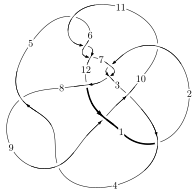
\includegraphics[width=112pt]{../../../GIT/diagram.site/Diagrams/png/1872_12a_1071.png}\\
\ \ \ A knot diagram\footnotemark}&
\allowdisplaybreaks
\textbf{Linearized knot diagam} \\
\cline{2-2}
 &
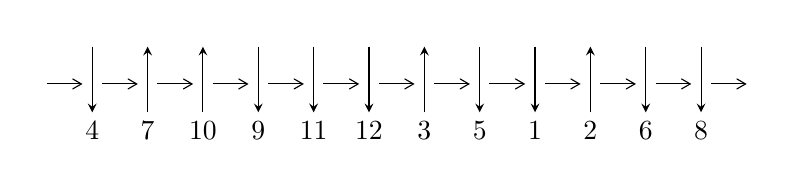
\begin{tikzpicture}[x=20pt, y=17pt]
	% nodes
	\node (C0) at (0, 0) {};
	\node (C1) at (1, 0) {};
	\node (C1U) at (1, +1) {};
	\node (C1D) at (1, -1) {4};

	\node (C2) at (2, 0) {};
	\node (C2U) at (2, +1) {};
	\node (C2D) at (2, -1) {7};

	\node (C3) at (3, 0) {};
	\node (C3U) at (3, +1) {};
	\node (C3D) at (3, -1) {10};

	\node (C4) at (4, 0) {};
	\node (C4U) at (4, +1) {};
	\node (C4D) at (4, -1) {9};

	\node (C5) at (5, 0) {};
	\node (C5U) at (5, +1) {};
	\node (C5D) at (5, -1) {11};

	\node (C6) at (6, 0) {};
	\node (C6U) at (6, +1) {};
	\node (C6D) at (6, -1) {12};

	\node (C7) at (7, 0) {};
	\node (C7U) at (7, +1) {};
	\node (C7D) at (7, -1) {3};

	\node (C8) at (8, 0) {};
	\node (C8U) at (8, +1) {};
	\node (C8D) at (8, -1) {5};

	\node (C9) at (9, 0) {};
	\node (C9U) at (9, +1) {};
	\node (C9D) at (9, -1) {1};

	\node (C10) at (10, 0) {};
	\node (C10U) at (10, +1) {};
	\node (C10D) at (10, -1) {2};

	\node (C11) at (11, 0) {};
	\node (C11U) at (11, +1) {};
	\node (C11D) at (11, -1) {6};

	\node (C12) at (12, 0) {};
	\node (C12U) at (12, +1) {};
	\node (C12D) at (12, -1) {8};
	\node (C13) at (13, 0) {};

	% arrows
	\draw[->,>={angle 60}]
	(C0) edge (C1) (C1) edge (C2) (C2) edge (C3) (C3) edge (C4) (C4) edge (C5) (C5) edge (C6) (C6) edge (C7) (C7) edge (C8) (C8) edge (C9) (C9) edge (C10) (C10) edge (C11) (C11) edge (C12) (C12) edge (C13) ;	\draw[->,>=stealth]
	(C1U) edge (C1D) (C2D) edge (C2U) (C3D) edge (C3U) (C4U) edge (C4D) (C5U) edge (C5D) (C6U) edge (C6D) (C7D) edge (C7U) (C8U) edge (C8D) (C9U) edge (C9D) (C10D) edge (C10U) (C11U) edge (C11D) (C12U) edge (C12D) ;
	\end{tikzpicture} \\
\hhline{~~} \\& 
\textbf{Solving Sequence} \\ \cline{2-2} 
 &
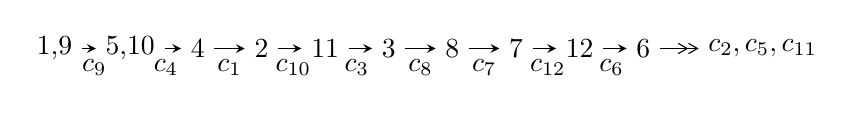
\begin{tikzpicture}[x=23pt, y=7pt]
	% node
	\node (A0) at (-1/8, 0) {1,9};
	\node (A1) at (17/16, 0) {5,10};
	\node (A2) at (17/8, 0) {4};
	\node (A3) at (25/8, 0) {2};
	\node (A4) at (33/8, 0) {11};
	\node (A5) at (41/8, 0) {3};
	\node (A6) at (49/8, 0) {8};
	\node (A7) at (57/8, 0) {7};
	\node (A8) at (65/8, 0) {12};
	\node (A9) at (73/8, 0) {6};
	\node (C1) at (1/2, -1) {$c_{9}$};
	\node (C2) at (13/8, -1) {$c_{4}$};
	\node (C3) at (21/8, -1) {$c_{1}$};
	\node (C4) at (29/8, -1) {$c_{10}$};
	\node (C5) at (37/8, -1) {$c_{3}$};
	\node (C6) at (45/8, -1) {$c_{8}$};
	\node (C7) at (53/8, -1) {$c_{7}$};
	\node (C8) at (61/8, -1) {$c_{12}$};
	\node (C9) at (69/8, -1) {$c_{6}$};
	\node (A10) at (11, 0) {$c_{2},c_{5},c_{11}$};

	% edge
	\draw[->,>=stealth]	
	(A0) edge (A1) (A1) edge (A2) (A2) edge (A3) (A3) edge (A4) (A4) edge (A5) (A5) edge (A6) (A6) edge (A7) (A7) edge (A8) (A8) edge (A9) ;
	\draw[->>,>={angle 60}]	
	(A9) edge (A10);
\end{tikzpicture} \\ 

\end{tabular} \\

\footnotetext{
The image of knot diagram is generated by the software ``\textbf{Draw programme}" developed by Andrew Bartholomew(\url{http://www.layer8.co.uk/maths/draw/index.htm\#Running-draw}), where we modified some parts for our purpose(\url{https://github.com/CATsTAILs/LinksPainter}).
}\phantom \\ \newline 
\centering \textbf{Ideals for irreducible components\footnotemark of $X_{\text{par}}$} 
 
\begin{align*}
I^u_{1}&=\langle 
1.77660\times10^{1245} u^{148}+6.71415\times10^{1245} u^{147}+\cdots+3.74457\times10^{1246} b+4.40626\times10^{1246},\\
\phantom{I^u_{1}}&\phantom{= \langle  }-8.25994\times10^{1246} u^{148}-3.27069\times10^{1247} u^{147}+\cdots+7.11469\times10^{1247} a-7.83372\times10^{1248},\\
\phantom{I^u_{1}}&\phantom{= \langle  }u^{149}+4 u^{148}+\cdots+73 u+19\rangle \\
I^u_{2}&=\langle 
3.40750\times10^{59} u^{37}-4.78008\times10^{59} u^{36}+\cdots+2.11717\times10^{60} b+2.49956\times10^{60},\\
\phantom{I^u_{2}}&\phantom{= \langle  }1.11713\times10^{60} u^{37}+5.75954\times10^{59} u^{36}+\cdots+2.11717\times10^{60} a+3.00294\times10^{59},\;u^{38}+u^{37}+\cdots+u+1\rangle \\
\\
\end{align*}
\raggedright * 2 irreducible components of $\dim_{\mathbb{C}}=0$, with total 187 representations.\\
\footnotetext{All coefficients of polynomials are rational numbers. But the coefficients are sometimes approximated in decimal forms when there is not enough margin.}
\newpage
\renewcommand{\arraystretch}{1}
\centering \section*{I. $I^u_{1}= \langle 1.78\times10^{1245} u^{148}+6.71\times10^{1245} u^{147}+\cdots+3.74\times10^{1246} b+4.41\times10^{1246},\;-8.26\times10^{1246} u^{148}-3.27\times10^{1247} u^{147}+\cdots+7.11\times10^{1247} a-7.83\times10^{1248},\;u^{149}+4 u^{148}+\cdots+73 u+19 \rangle$}
\flushleft \textbf{(i) Arc colorings}\\
\begin{tabular}{m{7pt} m{180pt} m{7pt} m{180pt} }
\flushright $a_{1}=$&$\begin{pmatrix}0\\u\end{pmatrix}$ \\
\flushright $a_{9}=$&$\begin{pmatrix}1\\0\end{pmatrix}$ \\
\flushright $a_{5}=$&$\begin{pmatrix}0.116097 u^{148}+0.459709 u^{147}+\cdots+40.4995 u+11.0106\\-0.0474446 u^{148}-0.179304 u^{147}+\cdots-10.7177 u-1.17671\end{pmatrix}$ \\
\flushright $a_{10}=$&$\begin{pmatrix}1\\u^2\end{pmatrix}$ \\
\flushright $a_{4}=$&$\begin{pmatrix}0.0686524 u^{148}+0.280405 u^{147}+\cdots+29.7818 u+9.83393\\-0.0474446 u^{148}-0.179304 u^{147}+\cdots-10.7177 u-1.17671\end{pmatrix}$ \\
\flushright $a_{2}=$&$\begin{pmatrix}-0.186978 u^{148}-0.641792 u^{147}+\cdots-24.8565 u+8.19043\\0.00844573 u^{148}-0.0141488 u^{147}+\cdots-15.8056 u-7.69389\end{pmatrix}$ \\
\flushright $a_{11}=$&$\begin{pmatrix}0.00409401 u^{148}+0.146299 u^{147}+\cdots+17.3491 u+25.6214\\-0.0900120 u^{148}-0.368345 u^{147}+\cdots-23.8847 u-6.46783\end{pmatrix}$ \\
\flushright $a_{3}=$&$\begin{pmatrix}0.123082 u^{148}+0.486614 u^{147}+\cdots+38.7720 u+10.9005\\-0.0540469 u^{148}-0.202096 u^{147}+\cdots-10.9116 u-0.958002\end{pmatrix}$ \\
\flushright $a_{8}=$&$\begin{pmatrix}0.381708 u^{148}+1.49767 u^{147}+\cdots+76.5844 u+9.83207\\0.0232331 u^{148}+0.130543 u^{147}+\cdots+8.11317 u+3.92302\end{pmatrix}$ \\
\flushright $a_{7}=$&$\begin{pmatrix}0.492860 u^{148}+1.91718 u^{147}+\cdots+107.856 u+14.4413\\-0.102583 u^{148}-0.381654 u^{147}+\cdots-19.7050 u+1.13749\end{pmatrix}$ \\
\flushright $a_{12}=$&$\begin{pmatrix}-0.290140 u^{148}-0.970062 u^{147}+\cdots-14.3930 u+25.9448\\-0.106358 u^{148}-0.443882 u^{147}+\cdots-27.3949 u-10.0581\end{pmatrix}$ \\
\flushright $a_{6}=$&$\begin{pmatrix}-0.0591855 u^{148}-0.0201284 u^{147}+\cdots+40.0677 u+41.7863\\-0.194071 u^{148}-0.782151 u^{147}+\cdots-45.3045 u-12.0010\end{pmatrix}$\\&\end{tabular}
\flushleft \textbf{(ii) Obstruction class $= -1$}\\~\\
\flushleft \textbf{(iii) Cusp Shapes $= 0.147174 u^{148}+0.542286 u^{147}+\cdots+1.94409 u-6.94054$}\\~\\
\newpage\renewcommand{\arraystretch}{1}
\flushleft \textbf{(iv) u-Polynomials at the component}\newline \\
\begin{tabular}{m{50pt}|m{274pt}}
Crossings & \hspace{64pt}u-Polynomials at each crossing \\
\hline $$\begin{aligned}c_{1}\end{aligned}$$&$\begin{aligned}
&u^{149}-10 u^{148}+\cdots+347212 u-23201
\end{aligned}$\\
\hline $$\begin{aligned}c_{2},c_{7}\end{aligned}$$&$\begin{aligned}
&u^{149}+2 u^{148}+\cdots-24326 u+7187
\end{aligned}$\\
\hline $$\begin{aligned}c_{3}\end{aligned}$$&$\begin{aligned}
&u^{149}+u^{148}+\cdots+u+1
\end{aligned}$\\
\hline $$\begin{aligned}c_{4},c_{8}\end{aligned}$$&$\begin{aligned}
&u^{149}+4 u^{148}+\cdots+163388 u+15389
\end{aligned}$\\
\hline $$\begin{aligned}c_{5},c_{6},c_{11}\end{aligned}$$&$\begin{aligned}
&u^{149}+u^{148}+\cdots-4044 u+667
\end{aligned}$\\
\hline $$\begin{aligned}c_{9}\end{aligned}$$&$\begin{aligned}
&u^{149}+4 u^{148}+\cdots+73 u+19
\end{aligned}$\\
\hline $$\begin{aligned}c_{10}\end{aligned}$$&$\begin{aligned}
&u^{149}+4 u^{148}+\cdots-116639488 u+34307711
\end{aligned}$\\
\hline $$\begin{aligned}c_{12}\end{aligned}$$&$\begin{aligned}
&u^{149}+u^{148}+\cdots-3432 u+23659
\end{aligned}$\\
\hline
\end{tabular}\\~\\
\newpage\renewcommand{\arraystretch}{1}
\flushleft \textbf{(v) Riley Polynomials at the component}\newline \\
\begin{tabular}{m{50pt}|m{274pt}}
Crossings & \hspace{64pt}Riley Polynomials at each crossing \\
\hline $$\begin{aligned}c_{1}\end{aligned}$$&$\begin{aligned}
&y^{149}+34 y^{148}+\cdots-32477715860 y-538286401
\end{aligned}$\\
\hline $$\begin{aligned}c_{2},c_{7}\end{aligned}$$&$\begin{aligned}
&y^{149}-80 y^{148}+\cdots+2042752080 y-51652969
\end{aligned}$\\
\hline $$\begin{aligned}c_{3}\end{aligned}$$&$\begin{aligned}
&y^{149}+15 y^{148}+\cdots-27 y-1
\end{aligned}$\\
\hline $$\begin{aligned}c_{4},c_{8}\end{aligned}$$&$\begin{aligned}
&y^{149}+110 y^{148}+\cdots-12741844090 y-236821321
\end{aligned}$\\
\hline $$\begin{aligned}c_{5},c_{6},c_{11}\end{aligned}$$&$\begin{aligned}
&y^{149}-141 y^{148}+\cdots-16078272 y-444889
\end{aligned}$\\
\hline $$\begin{aligned}c_{9}\end{aligned}$$&$\begin{aligned}
&y^{149}+28 y^{148}+\cdots-10593 y-361
\end{aligned}$\\
\hline $$\begin{aligned}c_{10}\end{aligned}$$&$\begin{aligned}
&y^{149}-12 y^{148}+\cdots+25050115881431194 y-1177019034059521
\end{aligned}$\\
\hline $$\begin{aligned}c_{12}\end{aligned}$$&$\begin{aligned}
&y^{149}+3 y^{148}+\cdots+13696191542 y-559748281
\end{aligned}$\\
\hline
\end{tabular}\\~\\
\newpage\flushleft \textbf{(vi) Complex Volumes and Cusp Shapes}
$$\begin{array}{c|c|c}  
\text{Solutions to }I^u_{1}& \I (\text{vol} + \sqrt{-1}CS) & \text{Cusp shape}\\
 \hline 
\begin{aligned}
u &= \phantom{-}0.822791 + 0.566488 I \\
a &= \phantom{-}0.044387 - 0.717158 I \\
b &= -0.912414 + 0.652071 I\end{aligned}
 & -6.14043 + 2.41887 I & \phantom{-0.000000 } 0 \\ \hline\begin{aligned}
u &= \phantom{-}0.822791 - 0.566488 I \\
a &= \phantom{-}0.044387 + 0.717158 I \\
b &= -0.912414 - 0.652071 I\end{aligned}
 & -6.14043 - 2.41887 I & \phantom{-0.000000 } 0 \\ \hline\begin{aligned}
u &= \phantom{-}0.684487 + 0.702737 I \\
a &= \phantom{-}0.250571 - 1.362020 I \\
b &= \phantom{-}0.00643 + 1.64717 I\end{aligned}
 & \phantom{-}0.17185 - 1.66565 I & \phantom{-0.000000 } 0 \\ \hline\begin{aligned}
u &= \phantom{-}0.684487 - 0.702737 I \\
a &= \phantom{-}0.250571 + 1.362020 I \\
b &= \phantom{-}0.00643 - 1.64717 I\end{aligned}
 & \phantom{-}0.17185 + 1.66565 I & \phantom{-0.000000 } 0 \\ \hline\begin{aligned}
u &= -0.641687 + 0.792516 I \\
a &= -0.232348 - 1.226240 I \\
b &= -0.33350 + 1.39920 I\end{aligned}
 & \phantom{-}3.07150 + 2.81514 I & \phantom{-0.000000 } 0 \\ \hline\begin{aligned}
u &= -0.641687 - 0.792516 I \\
a &= -0.232348 + 1.226240 I \\
b &= -0.33350 - 1.39920 I\end{aligned}
 & \phantom{-}3.07150 - 2.81514 I & \phantom{-0.000000 } 0 \\ \hline\begin{aligned}
u &= \phantom{-}0.556712 + 0.869557 I \\
a &= \phantom{-}1.91956 - 1.09013 I \\
b &= \phantom{-}0.028314 + 1.005700 I\end{aligned}
 & \phantom{-}3.26290 - 3.19090 I & \phantom{-0.000000 } 0 \\ \hline\begin{aligned}
u &= \phantom{-}0.556712 - 0.869557 I \\
a &= \phantom{-}1.91956 + 1.09013 I \\
b &= \phantom{-}0.028314 - 1.005700 I\end{aligned}
 & \phantom{-}3.26290 + 3.19090 I & \phantom{-0.000000 } 0 \\ \hline\begin{aligned}
u &= \phantom{-}0.712704 + 0.620664 I \\
a &= -0.529672 + 0.671924 I \\
b &= \phantom{-}1.191280 - 0.507002 I\end{aligned}
 & -7.60678 - 0.81095 I & \phantom{-0.000000 } 0 \\ \hline\begin{aligned}
u &= \phantom{-}0.712704 - 0.620664 I \\
a &= -0.529672 - 0.671924 I \\
b &= \phantom{-}1.191280 + 0.507002 I\end{aligned}
 & -7.60678 + 0.81095 I & \phantom{-0.000000 } 0\\
 \hline 
 \end{array}$$\newpage$$\begin{array}{c|c|c}  
\text{Solutions to }I^u_{1}& \I (\text{vol} + \sqrt{-1}CS) & \text{Cusp shape}\\
 \hline 
\begin{aligned}
u &= -0.740114 + 0.574065 I \\
a &= -0.1021720 - 0.0224356 I \\
b &= \phantom{-}1.370960 - 0.000930 I\end{aligned}
 & -7.36674 + 6.08958 I & \phantom{-0.000000 } 0 \\ \hline\begin{aligned}
u &= -0.740114 - 0.574065 I \\
a &= -0.1021720 + 0.0224356 I \\
b &= \phantom{-}1.370960 + 0.000930 I\end{aligned}
 & -7.36674 - 6.08958 I & \phantom{-0.000000 } 0 \\ \hline\begin{aligned}
u &= \phantom{-}0.909823 + 0.208880 I \\
a &= \phantom{-}0.076887 - 0.857113 I \\
b &= \phantom{-}0.521071 - 0.246570 I\end{aligned}
 & \phantom{-}1.16655 - 3.31820 I & \phantom{-0.000000 } 0 \\ \hline\begin{aligned}
u &= \phantom{-}0.909823 - 0.208880 I \\
a &= \phantom{-}0.076887 + 0.857113 I \\
b &= \phantom{-}0.521071 + 0.246570 I\end{aligned}
 & \phantom{-}1.16655 + 3.31820 I & \phantom{-0.000000 } 0 \\ \hline\begin{aligned}
u &= -0.784235 + 0.473889 I \\
a &= \phantom{-}0.380299 - 0.660353 I \\
b &= \phantom{-}0.663142 + 0.352778 I\end{aligned}
 & -1.01300 + 1.08677 I & \phantom{-0.000000 } 0 \\ \hline\begin{aligned}
u &= -0.784235 - 0.473889 I \\
a &= \phantom{-}0.380299 + 0.660353 I \\
b &= \phantom{-}0.663142 - 0.352778 I\end{aligned}
 & -1.01300 - 1.08677 I & \phantom{-0.000000 } 0 \\ \hline\begin{aligned}
u &= \phantom{-}0.555083 + 0.728859 I \\
a &= \phantom{-}0.055058 - 1.204150 I \\
b &= \phantom{-}0.66833 + 1.49831 I\end{aligned}
 & -2.51266 - 5.39632 I & \phantom{-0.000000 } 0 \\ \hline\begin{aligned}
u &= \phantom{-}0.555083 - 0.728859 I \\
a &= \phantom{-}0.055058 + 1.204150 I \\
b &= \phantom{-}0.66833 - 1.49831 I\end{aligned}
 & -2.51266 + 5.39632 I & \phantom{-0.000000 } 0 \\ \hline\begin{aligned}
u &= -0.914640 + 0.008017 I \\
a &= -0.250572 - 0.138236 I \\
b &= -0.602304 - 0.012616 I\end{aligned}
 & -1.092020 + 0.014144 I & \phantom{-0.000000 } 0 \\ \hline\begin{aligned}
u &= -0.914640 - 0.008017 I \\
a &= -0.250572 + 0.138236 I \\
b &= -0.602304 + 0.012616 I\end{aligned}
 & -1.092020 - 0.014144 I & \phantom{-0.000000 } 0\\
 \hline 
 \end{array}$$\newpage$$\begin{array}{c|c|c}  
\text{Solutions to }I^u_{1}& \I (\text{vol} + \sqrt{-1}CS) & \text{Cusp shape}\\
 \hline 
\begin{aligned}
u &= \phantom{-}0.731838 + 0.545147 I \\
a &= -0.193433 - 0.016628 I \\
b &= -1.062520 - 0.136919 I\end{aligned}
 & -1.84016 - 3.70908 I & \phantom{-0.000000 } 0 \\ \hline\begin{aligned}
u &= \phantom{-}0.731838 - 0.545147 I \\
a &= -0.193433 + 0.016628 I \\
b &= -1.062520 + 0.136919 I\end{aligned}
 & -1.84016 + 3.70908 I & \phantom{-0.000000 } 0 \\ \hline\begin{aligned}
u &= \phantom{-}0.347179 + 1.032320 I \\
a &= -0.202267 + 1.398820 I \\
b &= -0.68947 - 1.43468 I\end{aligned}
 & \phantom{-}1.46037 - 10.80160 I & \phantom{-0.000000 } 0 \\ \hline\begin{aligned}
u &= \phantom{-}0.347179 - 1.032320 I \\
a &= -0.202267 - 1.398820 I \\
b &= -0.68947 + 1.43468 I\end{aligned}
 & \phantom{-}1.46037 + 10.80160 I & \phantom{-0.000000 } 0 \\ \hline\begin{aligned}
u &= \phantom{-}0.404945 + 1.018820 I \\
a &= -0.959555 + 0.809393 I \\
b &= -0.028656 - 0.343001 I\end{aligned}
 & -5.06271 - 2.99689 I & \phantom{-0.000000 } 0 \\ \hline\begin{aligned}
u &= \phantom{-}0.404945 - 1.018820 I \\
a &= -0.959555 - 0.809393 I \\
b &= -0.028656 + 0.343001 I\end{aligned}
 & -5.06271 + 2.99689 I & \phantom{-0.000000 } 0 \\ \hline\begin{aligned}
u &= -0.852504 + 0.295008 I \\
a &= \phantom{-}0.234306 - 1.239890 I \\
b &= -0.559603 - 0.441689 I\end{aligned}
 & -3.79545 + 6.56578 I & \phantom{-0.000000 } 0 \\ \hline\begin{aligned}
u &= -0.852504 - 0.295008 I \\
a &= \phantom{-}0.234306 + 1.239890 I \\
b &= -0.559603 + 0.441689 I\end{aligned}
 & -3.79545 - 6.56578 I & \phantom{-0.000000 } 0 \\ \hline\begin{aligned}
u &= -1.002830 + 0.448400 I \\
a &= -0.530112 - 1.002450 I \\
b &= -0.181425 + 1.238740 I\end{aligned}
 & \phantom{-}2.67786 + 2.86179 I & \phantom{-0.000000 } 0 \\ \hline\begin{aligned}
u &= -1.002830 - 0.448400 I \\
a &= -0.530112 + 1.002450 I \\
b &= -0.181425 - 1.238740 I\end{aligned}
 & \phantom{-}2.67786 - 2.86179 I & \phantom{-0.000000 } 0\\
 \hline 
 \end{array}$$\newpage$$\begin{array}{c|c|c}  
\text{Solutions to }I^u_{1}& \I (\text{vol} + \sqrt{-1}CS) & \text{Cusp shape}\\
 \hline 
\begin{aligned}
u &= -0.827165 + 0.732877 I \\
a &= \phantom{-}0.065449 + 0.399351 I \\
b &= -0.954242 - 0.148969 I\end{aligned}
 & \phantom{-}0.52778 + 4.02864 I & \phantom{-0.000000 } 0 \\ \hline\begin{aligned}
u &= -0.827165 - 0.732877 I \\
a &= \phantom{-}0.065449 - 0.399351 I \\
b &= -0.954242 + 0.148969 I\end{aligned}
 & \phantom{-}0.52778 - 4.02864 I & \phantom{-0.000000 } 0 \\ \hline\begin{aligned}
u &= \phantom{-}0.059435 + 1.123230 I \\
a &= -0.451872 - 0.783174 I \\
b &= -0.123028 + 0.175062 I\end{aligned}
 & \phantom{-}3.28868 + 4.01813 I & \phantom{-0.000000 } 0 \\ \hline\begin{aligned}
u &= \phantom{-}0.059435 - 1.123230 I \\
a &= -0.451872 + 0.783174 I \\
b &= -0.123028 - 0.175062 I\end{aligned}
 & \phantom{-}3.28868 - 4.01813 I & \phantom{-0.000000 } 0 \\ \hline\begin{aligned}
u &= -0.136752 + 1.117670 I \\
a &= -0.004680 + 1.318210 I \\
b &= -0.659862 - 1.135610 I\end{aligned}
 & \phantom{-}4.32831 - 0.18892 I & \phantom{-0.000000 } 0 \\ \hline\begin{aligned}
u &= -0.136752 - 1.117670 I \\
a &= -0.004680 - 1.318210 I \\
b &= -0.659862 + 1.135610 I\end{aligned}
 & \phantom{-}4.32831 + 0.18892 I & \phantom{-0.000000 } 0 \\ \hline\begin{aligned}
u &= -0.567264 + 0.981487 I \\
a &= -1.51309 - 1.55737 I \\
b &= -0.103630 + 1.215780 I\end{aligned}
 & \phantom{-}7.04562 + 5.07163 I & \phantom{-0.000000 } 0 \\ \hline\begin{aligned}
u &= -0.567264 - 0.981487 I \\
a &= -1.51309 + 1.55737 I \\
b &= -0.103630 - 1.215780 I\end{aligned}
 & \phantom{-}7.04562 - 5.07163 I & \phantom{-0.000000 } 0 \\ \hline\begin{aligned}
u &= \phantom{-}0.856339 + 0.744503 I \\
a &= -0.0741008 + 0.0814312 I \\
b &= \phantom{-}1.107120 + 0.073780 I\end{aligned}
 & \phantom{-}1.29255 - 9.14879 I & \phantom{-0.000000 } 0 \\ \hline\begin{aligned}
u &= \phantom{-}0.856339 - 0.744503 I \\
a &= -0.0741008 - 0.0814312 I \\
b &= \phantom{-}1.107120 - 0.073780 I\end{aligned}
 & \phantom{-}1.29255 + 9.14879 I & \phantom{-0.000000 } 0\\
 \hline 
 \end{array}$$\newpage$$\begin{array}{c|c|c}  
\text{Solutions to }I^u_{1}& \I (\text{vol} + \sqrt{-1}CS) & \text{Cusp shape}\\
 \hline 
\begin{aligned}
u &= -0.193727 + 1.118850 I \\
a &= \phantom{-}0.146515 + 1.372280 I \\
b &= \phantom{-}0.62993 - 1.32351 I\end{aligned}
 & \phantom{-}6.87557 + 5.98406 I & \phantom{-0.000000 } 0 \\ \hline\begin{aligned}
u &= -0.193727 - 1.118850 I \\
a &= \phantom{-}0.146515 - 1.372280 I \\
b &= \phantom{-}0.62993 + 1.32351 I\end{aligned}
 & \phantom{-}6.87557 - 5.98406 I & \phantom{-0.000000 } 0 \\ \hline\begin{aligned}
u &= \phantom{-}1.016100 + 0.510997 I \\
a &= -1.029400 - 0.247265 I \\
b &= \phantom{-}0.145981 - 0.973278 I\end{aligned}
 & -3.94520 + 0.52520 I & \phantom{-0.000000 } 0 \\ \hline\begin{aligned}
u &= \phantom{-}1.016100 - 0.510997 I \\
a &= -1.029400 + 0.247265 I \\
b &= \phantom{-}0.145981 + 0.973278 I\end{aligned}
 & -3.94520 - 0.52520 I & \phantom{-0.000000 } 0 \\ \hline\begin{aligned}
u &= \phantom{-}1.081810 + 0.393115 I \\
a &= -0.432295 + 0.129104 I \\
b &= \phantom{-}0.933297 - 0.166898 I\end{aligned}
 & -8.43281 - 0.35878 I & \phantom{-0.000000 } 0 \\ \hline\begin{aligned}
u &= \phantom{-}1.081810 - 0.393115 I \\
a &= -0.432295 - 0.129104 I \\
b &= \phantom{-}0.933297 + 0.166898 I\end{aligned}
 & -8.43281 + 0.35878 I & \phantom{-0.000000 } 0 \\ \hline\begin{aligned}
u &= -0.881392 + 0.750525 I \\
a &= \phantom{-}0.214038 - 0.055567 I \\
b &= -1.280300 + 0.108912 I\end{aligned}
 & -4.84553 + 13.14190 I & \phantom{-0.000000 } 0 \\ \hline\begin{aligned}
u &= -0.881392 - 0.750525 I \\
a &= \phantom{-}0.214038 + 0.055567 I \\
b &= -1.280300 - 0.108912 I\end{aligned}
 & -4.84553 - 13.14190 I & \phantom{-0.000000 } 0 \\ \hline\begin{aligned}
u &= \phantom{-}0.219710 + 0.801720 I \\
a &= \phantom{-}0.098679 - 0.522747 I \\
b &= \phantom{-}0.892532 + 0.181824 I\end{aligned}
 & \phantom{-}3.72750 + 0.10143 I & \phantom{-0.000000 } 0 \\ \hline\begin{aligned}
u &= \phantom{-}0.219710 - 0.801720 I \\
a &= \phantom{-}0.098679 + 0.522747 I \\
b &= \phantom{-}0.892532 - 0.181824 I\end{aligned}
 & \phantom{-}3.72750 - 0.10143 I & \phantom{-0.000000 } 0\\
 \hline 
 \end{array}$$\newpage$$\begin{array}{c|c|c}  
\text{Solutions to }I^u_{1}& \I (\text{vol} + \sqrt{-1}CS) & \text{Cusp shape}\\
 \hline 
\begin{aligned}
u &= \phantom{-}0.506228 + 1.072760 I \\
a &= \phantom{-}1.37762 - 2.03261 I \\
b &= \phantom{-}0.057960 + 1.370180 I\end{aligned}
 & \phantom{-}2.25040 - 7.09751 I & \phantom{-0.000000 } 0 \\ \hline\begin{aligned}
u &= \phantom{-}0.506228 - 1.072760 I \\
a &= \phantom{-}1.37762 + 2.03261 I \\
b &= \phantom{-}0.057960 - 1.370180 I\end{aligned}
 & \phantom{-}2.25040 + 7.09751 I & \phantom{-0.000000 } 0 \\ \hline\begin{aligned}
u &= -0.591028 + 0.544821 I \\
a &= \phantom{-}0.482732 + 0.701730 I \\
b &= \phantom{-}1.054950 - 0.834211 I\end{aligned}
 & -4.85653 + 3.11200 I & \phantom{-0.000000 } 0 \\ \hline\begin{aligned}
u &= -0.591028 - 0.544821 I \\
a &= \phantom{-}0.482732 - 0.701730 I \\
b &= \phantom{-}1.054950 + 0.834211 I\end{aligned}
 & -4.85653 - 3.11200 I & \phantom{-0.000000 } 0 \\ \hline\begin{aligned}
u &= -0.776279 + 0.927653 I \\
a &= -0.777082 - 1.046550 I \\
b &= -0.603480 + 1.200590 I\end{aligned}
 & \phantom{-}4.28088 + 7.59415 I & \phantom{-0.000000 } 0 \\ \hline\begin{aligned}
u &= -0.776279 - 0.927653 I \\
a &= -0.777082 + 1.046550 I \\
b &= -0.603480 - 1.200590 I\end{aligned}
 & \phantom{-}4.28088 - 7.59415 I & \phantom{-0.000000 } 0 \\ \hline\begin{aligned}
u &= -1.158340 + 0.371013 I \\
a &= \phantom{-}0.597103 - 0.122745 I \\
b &= \phantom{-}0.094227 - 0.983239 I\end{aligned}
 & \phantom{-}0.73864 + 2.83022 I & \phantom{-0.000000 } 0 \\ \hline\begin{aligned}
u &= -1.158340 - 0.371013 I \\
a &= \phantom{-}0.597103 + 0.122745 I \\
b &= \phantom{-}0.094227 + 0.983239 I\end{aligned}
 & \phantom{-}0.73864 - 2.83022 I & \phantom{-0.000000 } 0 \\ \hline\begin{aligned}
u &= -0.319801 + 0.710569 I \\
a &= \phantom{-}0.132260 - 0.619108 I \\
b &= -1.232260 + 0.493503 I\end{aligned}
 & -1.91124 - 3.32706 I & \phantom{-0.000000 } 0 \\ \hline\begin{aligned}
u &= -0.319801 - 0.710569 I \\
a &= \phantom{-}0.132260 + 0.619108 I \\
b &= -1.232260 - 0.493503 I\end{aligned}
 & -1.91124 + 3.32706 I & \phantom{-0.000000 } 0\\
 \hline 
 \end{array}$$\newpage$$\begin{array}{c|c|c}  
\text{Solutions to }I^u_{1}& \I (\text{vol} + \sqrt{-1}CS) & \text{Cusp shape}\\
 \hline 
\begin{aligned}
u &= -0.988091 + 0.723363 I \\
a &= \phantom{-}0.183842 + 0.017986 I \\
b &= \phantom{-}0.478607 - 0.061501 I\end{aligned}
 & -1.08906 + 2.95891 I & \phantom{-0.000000 } 0 \\ \hline\begin{aligned}
u &= -0.988091 - 0.723363 I \\
a &= \phantom{-}0.183842 - 0.017986 I \\
b &= \phantom{-}0.478607 + 0.061501 I\end{aligned}
 & -1.08906 - 2.95891 I & \phantom{-0.000000 } 0 \\ \hline\begin{aligned}
u &= \phantom{-}1.234850 + 0.092095 I \\
a &= -0.188514 - 0.205299 I \\
b &= -0.248632 - 1.085570 I\end{aligned}
 & -2.98414 - 6.67124 I & \phantom{-0.000000 } 0 \\ \hline\begin{aligned}
u &= \phantom{-}1.234850 - 0.092095 I \\
a &= -0.188514 + 0.205299 I \\
b &= -0.248632 + 1.085570 I\end{aligned}
 & -2.98414 + 6.67124 I & \phantom{-0.000000 } 0 \\ \hline\begin{aligned}
u &= \phantom{-}0.763103 + 0.992115 I \\
a &= \phantom{-}0.83868 - 1.25890 I \\
b &= \phantom{-}0.439093 + 1.337560 I\end{aligned}
 & \phantom{-}8.26844 - 4.66889 I & \phantom{-0.000000 } 0 \\ \hline\begin{aligned}
u &= \phantom{-}0.763103 - 0.992115 I \\
a &= \phantom{-}0.83868 + 1.25890 I \\
b &= \phantom{-}0.439093 - 1.337560 I\end{aligned}
 & \phantom{-}8.26844 + 4.66889 I & \phantom{-0.000000 } 0 \\ \hline\begin{aligned}
u &= \phantom{-}0.690619 + 0.256098 I \\
a &= -1.134530 - 0.254755 I \\
b &= -0.601353 - 0.777995 I\end{aligned}
 & -0.92039 - 2.54804 I & \phantom{-0.000000 } 0 \\ \hline\begin{aligned}
u &= \phantom{-}0.690619 - 0.256098 I \\
a &= -1.134530 + 0.254755 I \\
b &= -0.601353 + 0.777995 I\end{aligned}
 & -0.92039 + 2.54804 I & \phantom{-0.000000 } 0 \\ \hline\begin{aligned}
u &= -0.735269\phantom{ +0.000000I} \\
a &= -0.0426728\phantom{ +0.000000I} \\
b &= -0.565864\phantom{ +0.000000I}\end{aligned}
 & -1.14530\phantom{ +0.000000I} & \phantom{-0.000000 } 0 \\ \hline\begin{aligned}
u &= -0.709645 + 0.024755 I \\
a &= \phantom{-}1.02958 - 1.25535 I \\
b &= \phantom{-}0.596020 - 0.915779 I\end{aligned}
 & -5.53049 + 0.84818 I & \phantom{-0.000000 } 0\\
 \hline 
 \end{array}$$\newpage$$\begin{array}{c|c|c}  
\text{Solutions to }I^u_{1}& \I (\text{vol} + \sqrt{-1}CS) & \text{Cusp shape}\\
 \hline 
\begin{aligned}
u &= -0.709645 - 0.024755 I \\
a &= \phantom{-}1.02958 + 1.25535 I \\
b &= \phantom{-}0.596020 + 0.915779 I\end{aligned}
 & -5.53049 - 0.84818 I & \phantom{-0.000000 } 0 \\ \hline\begin{aligned}
u &= -0.359244 + 1.263320 I \\
a &= \phantom{-}0.580321 - 1.010880 I \\
b &= -0.340106 + 0.264669 I\end{aligned}
 & -3.12866 - 7.48606 I & \phantom{-0.000000 } 0 \\ \hline\begin{aligned}
u &= -0.359244 - 1.263320 I \\
a &= \phantom{-}0.580321 + 1.010880 I \\
b &= -0.340106 - 0.264669 I\end{aligned}
 & -3.12866 + 7.48606 I & \phantom{-0.000000 } 0 \\ \hline\begin{aligned}
u &= -0.799300 + 1.053190 I \\
a &= -0.74196 - 1.36055 I \\
b &= -0.33684 + 1.45904 I\end{aligned}
 & \phantom{-}4.47048 + 1.63148 I & \phantom{-0.000000 } 0 \\ \hline\begin{aligned}
u &= -0.799300 - 1.053190 I \\
a &= -0.74196 + 1.36055 I \\
b &= -0.33684 - 1.45904 I\end{aligned}
 & \phantom{-}4.47048 - 1.63148 I & \phantom{-0.000000 } 0 \\ \hline\begin{aligned}
u &= -0.397807 + 0.532565 I \\
a &= -0.23162 - 2.56983 I \\
b &= -0.155695 + 1.056100 I\end{aligned}
 & \phantom{-}2.14947 + 2.63117 I & -4.00000 - 3.48885 I \\ \hline\begin{aligned}
u &= -0.397807 - 0.532565 I \\
a &= -0.23162 + 2.56983 I \\
b &= -0.155695 - 1.056100 I\end{aligned}
 & \phantom{-}2.14947 - 2.63117 I & -4.00000 + 3.48885 I \\ \hline\begin{aligned}
u &= \phantom{-}1.105120 + 0.877439 I \\
a &= \phantom{-}0.199968 + 0.016509 I \\
b &= -0.677538 + 0.208812 I\end{aligned}
 & -6.24761 - 4.45078 I & \phantom{-0.000000 } 0 \\ \hline\begin{aligned}
u &= \phantom{-}1.105120 - 0.877439 I \\
a &= \phantom{-}0.199968 - 0.016509 I \\
b &= -0.677538 - 0.208812 I\end{aligned}
 & -6.24761 + 4.45078 I & \phantom{-0.000000 } 0 \\ \hline\begin{aligned}
u &= -0.292532 + 0.505444 I \\
a &= \phantom{-}1.40602 - 0.60186 I \\
b &= \phantom{-}0.044037 - 1.048900 I\end{aligned}
 & \phantom{-}3.33827 - 2.84247 I & -1.76881 + 3.33646 I\\
 \hline 
 \end{array}$$\newpage$$\begin{array}{c|c|c}  
\text{Solutions to }I^u_{1}& \I (\text{vol} + \sqrt{-1}CS) & \text{Cusp shape}\\
 \hline 
\begin{aligned}
u &= -0.292532 - 0.505444 I \\
a &= \phantom{-}1.40602 + 0.60186 I \\
b &= \phantom{-}0.044037 + 1.048900 I\end{aligned}
 & \phantom{-}3.33827 + 2.84247 I & -1.76881 - 3.33646 I \\ \hline\begin{aligned}
u &= -1.08382 + 0.91193 I \\
a &= -0.300449 - 1.201790 I \\
b &= -0.222649 + 1.256110 I\end{aligned}
 & \phantom{-}2.75191 + 2.86034 I & \phantom{-0.000000 } 0 \\ \hline\begin{aligned}
u &= -1.08382 - 0.91193 I \\
a &= -0.300449 + 1.201790 I \\
b &= -0.222649 - 1.256110 I\end{aligned}
 & \phantom{-}2.75191 - 2.86034 I & \phantom{-0.000000 } 0 \\ \hline\begin{aligned}
u &= \phantom{-}0.01051 + 1.42451 I \\
a &= \phantom{-}0.299533 - 1.116610 I \\
b &= \phantom{-}0.162653 + 0.921564 I\end{aligned}
 & \phantom{-}3.33018 + 1.31474 I & \phantom{-0.000000 } 0 \\ \hline\begin{aligned}
u &= \phantom{-}0.01051 - 1.42451 I \\
a &= \phantom{-}0.299533 + 1.116610 I \\
b &= \phantom{-}0.162653 - 0.921564 I\end{aligned}
 & \phantom{-}3.33018 - 1.31474 I & \phantom{-0.000000 } 0 \\ \hline\begin{aligned}
u &= \phantom{-}0.116652 + 0.558197 I \\
a &= -2.24939 - 2.20309 I \\
b &= \phantom{-}0.250939 + 0.785151 I\end{aligned}
 & -4.36914 - 1.20866 I & -3.88970 + 4.69115 I \\ \hline\begin{aligned}
u &= \phantom{-}0.116652 - 0.558197 I \\
a &= -2.24939 + 2.20309 I \\
b &= \phantom{-}0.250939 - 0.785151 I\end{aligned}
 & -4.36914 + 1.20866 I & -3.88970 - 4.69115 I \\ \hline\begin{aligned}
u &= \phantom{-}0.71489 + 1.26705 I \\
a &= \phantom{-}0.437939 - 1.024770 I \\
b &= \phantom{-}0.032561 + 1.125830 I\end{aligned}
 & \phantom{-}3.47028 + 0.93146 I & \phantom{-0.000000 } 0 \\ \hline\begin{aligned}
u &= \phantom{-}0.71489 - 1.26705 I \\
a &= \phantom{-}0.437939 + 1.024770 I \\
b &= \phantom{-}0.032561 - 1.125830 I\end{aligned}
 & \phantom{-}3.47028 - 0.93146 I & \phantom{-0.000000 } 0 \\ \hline\begin{aligned}
u &= \phantom{-}0.535565 + 0.081022 I \\
a &= -1.68567 - 1.93268 I \\
b &= -0.387439 + 0.352998 I\end{aligned}
 & -5.03890 - 4.06980 I & -10.98331 - 1.05875 I\\
 \hline 
 \end{array}$$\newpage$$\begin{array}{c|c|c}  
\text{Solutions to }I^u_{1}& \I (\text{vol} + \sqrt{-1}CS) & \text{Cusp shape}\\
 \hline 
\begin{aligned}
u &= \phantom{-}0.535565 - 0.081022 I \\
a &= -1.68567 + 1.93268 I \\
b &= -0.387439 - 0.352998 I\end{aligned}
 & -5.03890 + 4.06980 I & -10.98331 + 1.05875 I \\ \hline\begin{aligned}
u &= \phantom{-}0.92278 + 1.13209 I \\
a &= -0.347640 + 0.920418 I \\
b &= -0.530799 - 0.800669 I\end{aligned}
 & -5.44631 - 2.90760 I & \phantom{-0.000000 } 0 \\ \hline\begin{aligned}
u &= \phantom{-}0.92278 - 1.13209 I \\
a &= -0.347640 - 0.920418 I \\
b &= -0.530799 + 0.800669 I\end{aligned}
 & -5.44631 + 2.90760 I & \phantom{-0.000000 } 0 \\ \hline\begin{aligned}
u &= -0.060516 + 0.532681 I \\
a &= -0.164411 + 0.444161 I \\
b &= -1.21016 - 1.05306 I\end{aligned}
 & \phantom{-}2.54178 + 1.17821 I & \phantom{-}11.64009 - 2.24509 I \\ \hline\begin{aligned}
u &= -0.060516 - 0.532681 I \\
a &= -0.164411 - 0.444161 I \\
b &= -1.21016 + 1.05306 I\end{aligned}
 & \phantom{-}2.54178 - 1.17821 I & \phantom{-}11.64009 + 2.24509 I \\ \hline\begin{aligned}
u &= \phantom{-}0.99166 + 1.11425 I \\
a &= -0.91295 + 1.42599 I \\
b &= -0.185960 - 1.394340 I\end{aligned}
 & \phantom{-}0.56601 - 4.83848 I & \phantom{-0.000000 } 0 \\ \hline\begin{aligned}
u &= \phantom{-}0.99166 - 1.11425 I \\
a &= -0.91295 - 1.42599 I \\
b &= -0.185960 + 1.394340 I\end{aligned}
 & \phantom{-}0.56601 + 4.83848 I & \phantom{-0.000000 } 0 \\ \hline\begin{aligned}
u &= -1.07785 + 1.05994 I \\
a &= \phantom{-}0.462928 + 1.232370 I \\
b &= \phantom{-}0.61542 - 1.40165 I\end{aligned}
 & -2.98411 + 12.81440 I & \phantom{-0.000000 } 0 \\ \hline\begin{aligned}
u &= -1.07785 - 1.05994 I \\
a &= \phantom{-}0.462928 - 1.232370 I \\
b &= \phantom{-}0.61542 + 1.40165 I\end{aligned}
 & -2.98411 - 12.81440 I & \phantom{-0.000000 } 0 \\ \hline\begin{aligned}
u &= \phantom{-}0.311732 + 0.358910 I \\
a &= \phantom{-}1.26566 - 4.52195 I \\
b &= \phantom{-}0.287040 + 1.083010 I\end{aligned}
 & \phantom{-}3.53857 - 6.53979 I & -2.29573 + 10.84804 I\\
 \hline 
 \end{array}$$\newpage$$\begin{array}{c|c|c}  
\text{Solutions to }I^u_{1}& \I (\text{vol} + \sqrt{-1}CS) & \text{Cusp shape}\\
 \hline 
\begin{aligned}
u &= \phantom{-}0.311732 - 0.358910 I \\
a &= \phantom{-}1.26566 + 4.52195 I \\
b &= \phantom{-}0.287040 - 1.083010 I\end{aligned}
 & \phantom{-}3.53857 + 6.53979 I & -2.29573 - 10.84804 I \\ \hline\begin{aligned}
u &= \phantom{-}1.10068 + 1.07688 I \\
a &= -0.497997 + 1.166620 I \\
b &= -0.49594 - 1.35858 I\end{aligned}
 & \phantom{-}2.72605 - 9.15496 I & \phantom{-0.000000 } 0 \\ \hline\begin{aligned}
u &= \phantom{-}1.10068 - 1.07688 I \\
a &= -0.497997 - 1.166620 I \\
b &= -0.49594 + 1.35858 I\end{aligned}
 & \phantom{-}2.72605 + 9.15496 I & \phantom{-0.000000 } 0 \\ \hline\begin{aligned}
u &= -0.019041 + 0.452582 I \\
a &= \phantom{-}0.718133 + 1.063210 I \\
b &= \phantom{-}0.70293 - 1.54683 I\end{aligned}
 & \phantom{-}5.29844 - 2.64181 I & \phantom{-}16.0425 + 10.8617 I \\ \hline\begin{aligned}
u &= -0.019041 - 0.452582 I \\
a &= \phantom{-}0.718133 - 1.063210 I \\
b &= \phantom{-}0.70293 + 1.54683 I\end{aligned}
 & \phantom{-}5.29844 + 2.64181 I & \phantom{-}16.0425 - 10.8617 I \\ \hline\begin{aligned}
u &= -0.245392 + 0.329056 I \\
a &= -0.98087 - 6.33078 I \\
b &= -0.345189 + 1.074550 I\end{aligned}
 & -1.91697 + 10.16090 I & -7.1460 - 13.4440 I \\ \hline\begin{aligned}
u &= -0.245392 - 0.329056 I \\
a &= -0.98087 + 6.33078 I \\
b &= -0.345189 - 1.074550 I\end{aligned}
 & -1.91697 - 10.16090 I & -7.1460 + 13.4440 I \\ \hline\begin{aligned}
u &= -0.208206 + 0.352641 I \\
a &= \phantom{-}1.83891 + 0.32050 I \\
b &= \phantom{-}0.149248 + 0.354691 I\end{aligned}
 & -0.326714 + 1.261040 I & -4.47886 - 3.96166 I \\ \hline\begin{aligned}
u &= -0.208206 - 0.352641 I \\
a &= \phantom{-}1.83891 - 0.32050 I \\
b &= \phantom{-}0.149248 - 0.354691 I\end{aligned}
 & -0.326714 - 1.261040 I & -4.47886 + 3.96166 I \\ \hline\begin{aligned}
u &= -0.001597 + 0.406180 I \\
a &= -0.45088 + 1.58611 I \\
b &= -0.66102 - 1.98194 I\end{aligned}
 & -0.18335 + 5.12037 I & \phantom{-}13.7772 - 4.9372 I\\
 \hline 
 \end{array}$$\newpage$$\begin{array}{c|c|c}  
\text{Solutions to }I^u_{1}& \I (\text{vol} + \sqrt{-1}CS) & \text{Cusp shape}\\
 \hline 
\begin{aligned}
u &= -0.001597 - 0.406180 I \\
a &= -0.45088 - 1.58611 I \\
b &= -0.66102 + 1.98194 I\end{aligned}
 & -0.18335 - 5.12037 I & \phantom{-}13.7772 + 4.9372 I \\ \hline\begin{aligned}
u &= \phantom{-}0.142368 + 0.376973 I \\
a &= -2.64476 + 0.71982 I \\
b &= -0.134828 - 1.375840 I\end{aligned}
 & \phantom{-}6.10118 + 0.21034 I & \phantom{-}4.82953 + 0.51502 I \\ \hline\begin{aligned}
u &= \phantom{-}0.142368 - 0.376973 I \\
a &= -2.64476 - 0.71982 I \\
b &= -0.134828 + 1.375840 I\end{aligned}
 & \phantom{-}6.10118 - 0.21034 I & \phantom{-}4.82953 - 0.51502 I \\ \hline\begin{aligned}
u &= \phantom{-}0.92096 + 1.31604 I \\
a &= \phantom{-}0.064604 - 1.199110 I \\
b &= \phantom{-}0.648507 + 1.063430 I\end{aligned}
 & -5.58238 - 7.08505 I & \phantom{-0.000000 } 0 \\ \hline\begin{aligned}
u &= \phantom{-}0.92096 - 1.31604 I \\
a &= \phantom{-}0.064604 + 1.199110 I \\
b &= \phantom{-}0.648507 - 1.063430 I\end{aligned}
 & -5.58238 + 7.08505 I & \phantom{-0.000000 } 0 \\ \hline\begin{aligned}
u &= -1.13004 + 1.14773 I \\
a &= \phantom{-}0.498632 + 1.050560 I \\
b &= \phantom{-}0.360295 - 1.201120 I\end{aligned}
 & \phantom{-}1.72436 + 4.88386 I & \phantom{-0.000000 } 0 \\ \hline\begin{aligned}
u &= -1.13004 - 1.14773 I \\
a &= \phantom{-}0.498632 - 1.050560 I \\
b &= \phantom{-}0.360295 + 1.201120 I\end{aligned}
 & \phantom{-}1.72436 - 4.88386 I & \phantom{-0.000000 } 0 \\ \hline\begin{aligned}
u &= -0.98295 + 1.31634 I \\
a &= -0.520381 - 0.851587 I \\
b &= \phantom{-}0.219731 + 1.105980 I\end{aligned}
 & -2.60212 - 4.67238 I & \phantom{-0.000000 } 0 \\ \hline\begin{aligned}
u &= -0.98295 - 1.31634 I \\
a &= -0.520381 + 0.851587 I \\
b &= \phantom{-}0.219731 - 1.105980 I\end{aligned}
 & -2.60212 + 4.67238 I & \phantom{-0.000000 } 0 \\ \hline\begin{aligned}
u &= -0.47592 + 1.57457 I \\
a &= -0.200625 - 1.006440 I \\
b &= -0.313934 + 0.854211 I\end{aligned}
 & \phantom{-}3.46409 + 4.38803 I & \phantom{-0.000000 } 0\\
 \hline 
 \end{array}$$\newpage$$\begin{array}{c|c|c}  
\text{Solutions to }I^u_{1}& \I (\text{vol} + \sqrt{-1}CS) & \text{Cusp shape}\\
 \hline 
\begin{aligned}
u &= -0.47592 - 1.57457 I \\
a &= -0.200625 + 1.006440 I \\
b &= -0.313934 - 0.854211 I\end{aligned}
 & \phantom{-}3.46409 - 4.38803 I & \phantom{-0.000000 } 0 \\ \hline\begin{aligned}
u &= -1.10913 + 1.22830 I \\
a &= -0.42349 - 1.37161 I \\
b &= -0.56727 + 1.43965 I\end{aligned}
 & -0.0057 + 19.5333 I & \phantom{-0.000000 } 0 \\ \hline\begin{aligned}
u &= -1.10913 - 1.22830 I \\
a &= -0.42349 + 1.37161 I \\
b &= -0.56727 - 1.43965 I\end{aligned}
 & -0.0057 - 19.5333 I & \phantom{-0.000000 } 0 \\ \hline\begin{aligned}
u &= -0.322870 + 0.079521 I \\
a &= \phantom{-}4.60389 + 1.60494 I \\
b &= \phantom{-}0.521329 - 0.712682 I\end{aligned}
 & -6.14357 + 3.72546 I & -15.6967 - 1.8148 I \\ \hline\begin{aligned}
u &= -0.322870 - 0.079521 I \\
a &= \phantom{-}4.60389 - 1.60494 I \\
b &= \phantom{-}0.521329 + 0.712682 I\end{aligned}
 & -6.14357 - 3.72546 I & -15.6967 + 1.8148 I \\ \hline\begin{aligned}
u &= -0.101421 + 0.314930 I \\
a &= \phantom{-}3.77657 + 2.32255 I \\
b &= \phantom{-}0.03817 - 1.46841 I\end{aligned}
 & \phantom{-}1.15038 + 2.98488 I & -1.23989 - 2.08887 I \\ \hline\begin{aligned}
u &= -0.101421 - 0.314930 I \\
a &= \phantom{-}3.77657 - 2.32255 I \\
b &= \phantom{-}0.03817 + 1.46841 I\end{aligned}
 & \phantom{-}1.15038 - 2.98488 I & -1.23989 + 2.08887 I \\ \hline\begin{aligned}
u &= \phantom{-}0.76399 + 1.51490 I \\
a &= -0.17722 + 1.73202 I \\
b &= -0.335847 - 1.204970 I\end{aligned}
 & -3.13095 - 8.20929 I & \phantom{-0.000000 } 0 \\ \hline\begin{aligned}
u &= \phantom{-}0.76399 - 1.51490 I \\
a &= -0.17722 - 1.73202 I \\
b &= -0.335847 + 1.204970 I\end{aligned}
 & -3.13095 + 8.20929 I & \phantom{-0.000000 } 0 \\ \hline\begin{aligned}
u &= \phantom{-}1.12979 + 1.26882 I \\
a &= \phantom{-}0.392036 - 1.293300 I \\
b &= \phantom{-}0.51917 + 1.38258 I\end{aligned}
 & \phantom{-}5.8399 - 14.8700 I & \phantom{-0.000000 } 0\\
 \hline 
 \end{array}$$\newpage$$\begin{array}{c|c|c}  
\text{Solutions to }I^u_{1}& \I (\text{vol} + \sqrt{-1}CS) & \text{Cusp shape}\\
 \hline 
\begin{aligned}
u &= \phantom{-}1.12979 - 1.26882 I \\
a &= \phantom{-}0.392036 + 1.293300 I \\
b &= \phantom{-}0.51917 - 1.38258 I\end{aligned}
 & \phantom{-}5.8399 + 14.8700 I & \phantom{-0.000000 } 0 \\ \hline\begin{aligned}
u &= -1.34716 + 1.07030 I \\
a &= \phantom{-}0.485580 + 1.072570 I \\
b &= \phantom{-}0.111570 - 1.379870 I\end{aligned}
 & \phantom{-}2.74353 + 5.90452 I & \phantom{-0.000000 } 0 \\ \hline\begin{aligned}
u &= -1.34716 - 1.07030 I \\
a &= \phantom{-}0.485580 - 1.072570 I \\
b &= \phantom{-}0.111570 + 1.379870 I\end{aligned}
 & \phantom{-}2.74353 - 5.90452 I & \phantom{-0.000000 } 0 \\ \hline\begin{aligned}
u &= \phantom{-}1.00526 + 1.41088 I \\
a &= \phantom{-}0.01130 - 1.49942 I \\
b &= \phantom{-}0.440065 + 1.245610 I\end{aligned}
 & -4.97260 - 5.23974 I & \phantom{-0.000000 } 0 \\ \hline\begin{aligned}
u &= \phantom{-}1.00526 - 1.41088 I \\
a &= \phantom{-}0.01130 + 1.49942 I \\
b &= \phantom{-}0.440065 - 1.245610 I\end{aligned}
 & -4.97260 + 5.23974 I & \phantom{-0.000000 } 0 \\ \hline\begin{aligned}
u &= -1.11452 + 1.35069 I \\
a &= -0.309636 - 1.220240 I \\
b &= -0.492999 + 1.279710 I\end{aligned}
 & \phantom{-}4.12884 + 9.22344 I & \phantom{-0.000000 } 0 \\ \hline\begin{aligned}
u &= -1.11452 - 1.35069 I \\
a &= -0.309636 + 1.220240 I \\
b &= -0.492999 - 1.279710 I\end{aligned}
 & \phantom{-}4.12884 - 9.22344 I & \phantom{-0.000000 } 0 \\ \hline\begin{aligned}
u &= -1.11423 + 1.38028 I \\
a &= \phantom{-}0.43755 + 1.41159 I \\
b &= \phantom{-}0.210804 - 1.289680 I\end{aligned}
 & \phantom{-}3.11861 + 5.61511 I & \phantom{-0.000000 } 0 \\ \hline\begin{aligned}
u &= -1.11423 - 1.38028 I \\
a &= \phantom{-}0.43755 - 1.41159 I \\
b &= \phantom{-}0.210804 + 1.289680 I\end{aligned}
 & \phantom{-}3.11861 - 5.61511 I & \phantom{-0.000000 } 0 \\ \hline\begin{aligned}
u &= \phantom{-}0.168788 + 0.117962 I \\
a &= -4.45602 + 3.79259 I \\
b &= -0.280598 - 0.840440 I\end{aligned}
 & -0.55056 - 1.50329 I & -8.82318 + 4.22354 I\\
 \hline 
 \end{array}$$\newpage$$\begin{array}{c|c|c}  
\text{Solutions to }I^u_{1}& \I (\text{vol} + \sqrt{-1}CS) & \text{Cusp shape}\\
 \hline 
\begin{aligned}
u &= \phantom{-}0.168788 - 0.117962 I \\
a &= -4.45602 - 3.79259 I \\
b &= -0.280598 + 0.840440 I\end{aligned}
 & -0.55056 + 1.50329 I & -8.82318 - 4.22354 I \\ \hline\begin{aligned}
u &= \phantom{-}1.93305 + 0.50959 I \\
a &= -0.142191 + 0.902871 I \\
b &= \phantom{-}0.066677 - 1.257350 I\end{aligned}
 & \phantom{-}5.77816 - 1.65318 I & \phantom{-0.000000 } 0 \\ \hline\begin{aligned}
u &= \phantom{-}1.93305 - 0.50959 I \\
a &= -0.142191 - 0.902871 I \\
b &= \phantom{-}0.066677 + 1.257350 I\end{aligned}
 & \phantom{-}5.77816 + 1.65318 I & \phantom{-0.000000 } 0 \\ \hline\begin{aligned}
u &= -1.06894 + 2.02788 I \\
a &= \phantom{-}0.327388 + 1.050300 I \\
b &= \phantom{-}0.013925 - 1.040450 I\end{aligned}
 & \phantom{-}3.88914 + 1.74878 I & \phantom{-0.000000 } 0 \\ \hline\begin{aligned}
u &= -1.06894 - 2.02788 I \\
a &= \phantom{-}0.327388 - 1.050300 I \\
b &= \phantom{-}0.013925 + 1.040450 I\end{aligned}
 & \phantom{-}3.88914 - 1.74878 I & \phantom{-0.000000 } 0 \\ \hline\begin{aligned}
u &= -1.66582 + 1.59423 I \\
a &= \phantom{-}0.348814 + 0.957220 I \\
b &= -0.230037 - 1.137420 I\end{aligned}
 & -0.55295 - 9.90422 I & \phantom{-0.000000 } 0 \\ \hline\begin{aligned}
u &= -1.66582 - 1.59423 I \\
a &= \phantom{-}0.348814 - 0.957220 I \\
b &= -0.230037 + 1.137420 I\end{aligned}
 & -0.55295 + 9.90422 I & \phantom{-0.000000 } 0 \\ \hline\begin{aligned}
u &= \phantom{-}1.40388 + 2.07476 I \\
a &= -0.297089 + 1.030670 I \\
b &= \phantom{-}0.090175 - 1.110300 I\end{aligned}
 & \phantom{-}5.54771 + 4.59569 I & \phantom{-0.000000 } 0 \\ \hline\begin{aligned}
u &= \phantom{-}1.40388 - 2.07476 I \\
a &= -0.297089 - 1.030670 I \\
b &= \phantom{-}0.090175 + 1.110300 I\end{aligned}
 & \phantom{-}5.54771 - 4.59569 I & \phantom{-0.000000 } 0\\
 \hline 
 \end{array}$$\newpage\newpage\renewcommand{\arraystretch}{1}
\centering \section*{II. $I^u_{2}= \langle 3.41\times10^{59} u^{37}-4.78\times10^{59} u^{36}+\cdots+2.12\times10^{60} b+2.50\times10^{60},\;1.12\times10^{60} u^{37}+5.76\times10^{59} u^{36}+\cdots+2.12\times10^{60} a+3.00\times10^{59},\;u^{38}+u^{37}+\cdots+u+1 \rangle$}
\flushleft \textbf{(i) Arc colorings}\\
\begin{tabular}{m{7pt} m{180pt} m{7pt} m{180pt} }
\flushright $a_{1}=$&$\begin{pmatrix}0\\u\end{pmatrix}$ \\
\flushright $a_{9}=$&$\begin{pmatrix}1\\0\end{pmatrix}$ \\
\flushright $a_{5}=$&$\begin{pmatrix}-0.527654 u^{37}-0.272040 u^{36}+\cdots+2.69562 u-0.141838\\-0.160946 u^{37}+0.225777 u^{36}+\cdots-3.74177 u-1.18061\end{pmatrix}$ \\
\flushright $a_{10}=$&$\begin{pmatrix}1\\u^2\end{pmatrix}$ \\
\flushright $a_{4}=$&$\begin{pmatrix}-0.688600 u^{37}-0.0462627 u^{36}+\cdots-1.04615 u-1.32245\\-0.160946 u^{37}+0.225777 u^{36}+\cdots-3.74177 u-1.18061\end{pmatrix}$ \\
\flushright $a_{2}=$&$\begin{pmatrix}-2.70490 u^{37}-1.58675 u^{36}+\cdots-2.58789 u-2.51374\\-1.06367 u^{37}-0.854375 u^{36}+\cdots+1.82410 u-0.789642\end{pmatrix}$ \\
\flushright $a_{11}=$&$\begin{pmatrix}1.80241 u^{37}+0.623202 u^{36}+\cdots+5.76280 u+0.911275\\0.223824 u^{37}+0.0376423 u^{36}+\cdots-0.954155 u-1.76154\end{pmatrix}$ \\
\flushright $a_{3}=$&$\begin{pmatrix}-0.894677 u^{37}-0.628125 u^{36}+\cdots+2.74189 u-0.784175\\0.281975 u^{37}+0.316543 u^{36}+\cdots-3.15991 u-0.804828\end{pmatrix}$ \\
\flushright $a_{8}=$&$\begin{pmatrix}0.0958034 u^{37}-0.488043 u^{36}+\cdots+1.03707 u+1.30515\\0.693839 u^{37}+0.214017 u^{36}+\cdots-0.197944 u+1.30859\end{pmatrix}$ \\
\flushright $a_{7}=$&$\begin{pmatrix}-0.274532 u^{37}-0.751509 u^{36}+\cdots-1.60654 u-0.419018\\0.416502 u^{37}+0.416592 u^{36}+\cdots+2.41842 u+2.42587\end{pmatrix}$ \\
\flushright $a_{12}=$&$\begin{pmatrix}-0.607657 u^{37}-0.0389698 u^{36}+\cdots-4.43061 u-1.64344\\-0.737209 u^{37}-0.936332 u^{36}+\cdots+4.58964 u+0.759813\end{pmatrix}$ \\
\flushright $a_{6}=$&$\begin{pmatrix}-1.69112 u^{37}-1.54813 u^{36}+\cdots-0.427166 u-2.14299\\0.0531670 u^{37}+0.360339 u^{36}+\cdots-6.98830 u-1.20508\end{pmatrix}$\\&\end{tabular}
\flushleft \textbf{(ii) Obstruction class $= 1$}\\~\\
\flushleft \textbf{(iii) Cusp Shapes $= 3.31222 u^{37}-0.0478282 u^{36}+\cdots-8.77444 u-13.9498$}\\~\\
\newpage\renewcommand{\arraystretch}{1}
\flushleft \textbf{(iv) u-Polynomials at the component}\newline \\
\begin{tabular}{m{50pt}|m{274pt}}
Crossings & \hspace{64pt}u-Polynomials at each crossing \\
\hline $$\begin{aligned}c_{1}\end{aligned}$$&$\begin{aligned}
&u^{38}-3 u^{37}+\cdots+8 u^2+1
\end{aligned}$\\
\hline $$\begin{aligned}c_{2}\end{aligned}$$&$\begin{aligned}
&u^{38}- u^{37}+\cdots-16 u^2+1
\end{aligned}$\\
\hline $$\begin{aligned}c_{3}\end{aligned}$$&$\begin{aligned}
&u^{38}+4 u^{36}+\cdots+u+1
\end{aligned}$\\
\hline $$\begin{aligned}c_{4}\end{aligned}$$&$\begin{aligned}
&u^{38}+u^{37}+\cdots-16 u+1
\end{aligned}$\\
\hline $$\begin{aligned}c_{5},c_{6}\end{aligned}$$&$\begin{aligned}
&u^{38}-20 u^{36}+\cdots+2 u+1
\end{aligned}$\\
\hline $$\begin{aligned}c_{7}\end{aligned}$$&$\begin{aligned}
&u^{38}+u^{37}+\cdots-16 u^2+1
\end{aligned}$\\
\hline $$\begin{aligned}c_{8}\end{aligned}$$&$\begin{aligned}
&u^{38}- u^{37}+\cdots+16 u+1
\end{aligned}$\\
\hline $$\begin{aligned}c_{9}\end{aligned}$$&$\begin{aligned}
&u^{38}+u^{37}+\cdots+u+1
\end{aligned}$\\
\hline $$\begin{aligned}c_{10}\end{aligned}$$&$\begin{aligned}
&u^{38}-5 u^{37}+\cdots-4 u+53
\end{aligned}$\\
\hline $$\begin{aligned}c_{11}\end{aligned}$$&$\begin{aligned}
&u^{38}-20 u^{36}+\cdots-2 u+1
\end{aligned}$\\
\hline $$\begin{aligned}c_{12}\end{aligned}$$&$\begin{aligned}
&u^{38}+6 u^{36}+\cdots-10 u+1
\end{aligned}$\\
\hline
\end{tabular}\\~\\
\newpage\renewcommand{\arraystretch}{1}
\flushleft \textbf{(v) Riley Polynomials at the component}\newline \\
\begin{tabular}{m{50pt}|m{274pt}}
Crossings & \hspace{64pt}Riley Polynomials at each crossing \\
\hline $$\begin{aligned}c_{1}\end{aligned}$$&$\begin{aligned}
&y^{38}+11 y^{37}+\cdots+16 y+1
\end{aligned}$\\
\hline $$\begin{aligned}c_{2},c_{7}\end{aligned}$$&$\begin{aligned}
&y^{38}-23 y^{37}+\cdots-32 y+1
\end{aligned}$\\
\hline $$\begin{aligned}c_{3}\end{aligned}$$&$\begin{aligned}
&y^{38}+8 y^{37}+\cdots+3 y+1
\end{aligned}$\\
\hline $$\begin{aligned}c_{4},c_{8}\end{aligned}$$&$\begin{aligned}
&y^{38}+35 y^{37}+\cdots-78 y+1
\end{aligned}$\\
\hline $$\begin{aligned}c_{5},c_{6},c_{11}\end{aligned}$$&$\begin{aligned}
&y^{38}-40 y^{37}+\cdots+8 y+1
\end{aligned}$\\
\hline $$\begin{aligned}c_{9}\end{aligned}$$&$\begin{aligned}
&y^{38}+17 y^{37}+\cdots-3 y+1
\end{aligned}$\\
\hline $$\begin{aligned}c_{10}\end{aligned}$$&$\begin{aligned}
&y^{38}+9 y^{37}+\cdots+52030 y+2809
\end{aligned}$\\
\hline $$\begin{aligned}c_{12}\end{aligned}$$&$\begin{aligned}
&y^{38}+12 y^{37}+\cdots-78 y+1
\end{aligned}$\\
\hline
\end{tabular}\\~\\
\newpage\flushleft \textbf{(vi) Complex Volumes and Cusp Shapes}
$$\begin{array}{c|c|c}  
\text{Solutions to }I^u_{2}& \I (\text{vol} + \sqrt{-1}CS) & \text{Cusp shape}\\
 \hline 
\begin{aligned}
u &= -0.581819 + 0.787198 I \\
a &= -1.90066 - 1.35846 I \\
b &= -0.233545 + 1.225910 I\end{aligned}
 & \phantom{-}3.84319 + 4.71088 I & -0.46280 - 6.88160 I \\ \hline\begin{aligned}
u &= -0.581819 - 0.787198 I \\
a &= -1.90066 + 1.35846 I \\
b &= -0.233545 - 1.225910 I\end{aligned}
 & \phantom{-}3.84319 - 4.71088 I & -0.46280 + 6.88160 I \\ \hline\begin{aligned}
u &= -0.809020 + 0.529699 I \\
a &= -0.574982 - 0.508391 I \\
b &= \phantom{-}1.062970 + 0.368148 I\end{aligned}
 & -7.65620 + 0.44843 I & -5.28310 + 6.52923 I \\ \hline\begin{aligned}
u &= -0.809020 - 0.529699 I \\
a &= -0.574982 + 0.508391 I \\
b &= \phantom{-}1.062970 - 0.368148 I\end{aligned}
 & -7.65620 - 0.44843 I & -5.28310 - 6.52923 I \\ \hline\begin{aligned}
u &= -0.770684 + 0.489111 I \\
a &= \phantom{-}1.209020 - 0.469475 I \\
b &= -0.1337560 - 0.0453600 I\end{aligned}
 & -4.73247 + 4.87232 I & -6.50156 - 6.48883 I \\ \hline\begin{aligned}
u &= -0.770684 - 0.489111 I \\
a &= \phantom{-}1.209020 + 0.469475 I \\
b &= -0.1337560 + 0.0453600 I\end{aligned}
 & -4.73247 - 4.87232 I & -6.50156 + 6.48883 I \\ \hline\begin{aligned}
u &= \phantom{-}0.952857 + 0.579267 I \\
a &= -0.267959 - 0.396124 I \\
b &= -0.391639 + 0.059254 I\end{aligned}
 & -0.87311 - 2.32740 I & -5.14628 + 1.05771 I \\ \hline\begin{aligned}
u &= \phantom{-}0.952857 - 0.579267 I \\
a &= -0.267959 + 0.396124 I \\
b &= -0.391639 - 0.059254 I\end{aligned}
 & -0.87311 + 2.32740 I & -5.14628 - 1.05771 I \\ \hline\begin{aligned}
u &= -0.168510 + 0.821634 I \\
a &= \phantom{-}0.450203 + 0.707128 I \\
b &= \phantom{-}0.440251 - 1.087420 I\end{aligned}
 & \phantom{-}4.80718 - 2.28673 I & \phantom{-}3.50663 + 1.43338 I \\ \hline\begin{aligned}
u &= -0.168510 - 0.821634 I \\
a &= \phantom{-}0.450203 - 0.707128 I \\
b &= \phantom{-}0.440251 + 1.087420 I\end{aligned}
 & \phantom{-}4.80718 + 2.28673 I & \phantom{-}3.50663 - 1.43338 I\\
 \hline 
 \end{array}$$\newpage$$\begin{array}{c|c|c}  
\text{Solutions to }I^u_{2}& \I (\text{vol} + \sqrt{-1}CS) & \text{Cusp shape}\\
 \hline 
\begin{aligned}
u &= \phantom{-}0.429288 + 1.103280 I \\
a &= \phantom{-}0.82581 - 1.88992 I \\
b &= -0.295937 + 1.059150 I\end{aligned}
 & -1.49530 + 9.25404 I & -3.65023 - 5.86849 I \\ \hline\begin{aligned}
u &= \phantom{-}0.429288 - 1.103280 I \\
a &= \phantom{-}0.82581 + 1.88992 I \\
b &= -0.295937 - 1.059150 I\end{aligned}
 & -1.49530 - 9.25404 I & -3.65023 + 5.86849 I \\ \hline\begin{aligned}
u &= -0.652127 + 0.477531 I \\
a &= -0.116840 + 0.569044 I \\
b &= \phantom{-}0.346306 - 1.290060 I\end{aligned}
 & \phantom{-}4.84984 - 2.43886 I & -0.90164 + 3.88333 I \\ \hline\begin{aligned}
u &= -0.652127 - 0.477531 I \\
a &= -0.116840 - 0.569044 I \\
b &= \phantom{-}0.346306 + 1.290060 I\end{aligned}
 & \phantom{-}4.84984 + 2.43886 I & -0.90164 - 3.88333 I \\ \hline\begin{aligned}
u &= \phantom{-}0.719715 + 0.342472 I \\
a &= -1.044510 - 0.281028 I \\
b &= -0.547744 - 0.636800 I\end{aligned}
 & -0.96062 - 2.81911 I & -6.3302 + 15.4084 I \\ \hline\begin{aligned}
u &= \phantom{-}0.719715 - 0.342472 I \\
a &= -1.044510 + 0.281028 I \\
b &= -0.547744 + 0.636800 I\end{aligned}
 & -0.96062 + 2.81911 I & -6.3302 - 15.4084 I \\ \hline\begin{aligned}
u &= -0.517454 + 0.528654 I \\
a &= \phantom{-}1.42791 + 1.11087 I \\
b &= \phantom{-}0.642884 - 0.618003 I\end{aligned}
 & -5.71245 + 4.31152 I & -8.79528 - 9.81076 I \\ \hline\begin{aligned}
u &= -0.517454 - 0.528654 I \\
a &= \phantom{-}1.42791 - 1.11087 I \\
b &= \phantom{-}0.642884 + 0.618003 I\end{aligned}
 & -5.71245 - 4.31152 I & -8.79528 + 9.81076 I \\ \hline\begin{aligned}
u &= \phantom{-}0.677000 + 1.142220 I \\
a &= \phantom{-}0.94945 - 1.31823 I \\
b &= \phantom{-}0.208074 + 1.176800 I\end{aligned}
 & \phantom{-}5.85215 - 5.01077 I & \phantom{-0.000000 -}0. + 4.64122 I \\ \hline\begin{aligned}
u &= \phantom{-}0.677000 - 1.142220 I \\
a &= \phantom{-}0.94945 + 1.31823 I \\
b &= \phantom{-}0.208074 - 1.176800 I\end{aligned}
 & \phantom{-}5.85215 + 5.01077 I & \phantom{-0.000000 } 0. - 4.64122 I\\
 \hline 
 \end{array}$$\newpage$$\begin{array}{c|c|c}  
\text{Solutions to }I^u_{2}& \I (\text{vol} + \sqrt{-1}CS) & \text{Cusp shape}\\
 \hline 
\begin{aligned}
u &= -0.659289 + 0.103010 I \\
a &= \phantom{-}0.67203 - 1.75898 I \\
b &= \phantom{-}0.539517 - 0.759509 I\end{aligned}
 & -5.47128 + 1.31809 I & -10.72815 - 9.07865 I \\ \hline\begin{aligned}
u &= -0.659289 - 0.103010 I \\
a &= \phantom{-}0.67203 + 1.75898 I \\
b &= \phantom{-}0.539517 + 0.759509 I\end{aligned}
 & -5.47128 - 1.31809 I & -10.72815 + 9.07865 I \\ \hline\begin{aligned}
u &= \phantom{-}0.063673 + 1.400840 I \\
a &= \phantom{-}0.004534 - 1.302700 I \\
b &= -0.351265 + 1.141000 I\end{aligned}
 & \phantom{-}3.52316 - 0.22029 I & \phantom{-0.000000 } 0 \\ \hline\begin{aligned}
u &= \phantom{-}0.063673 - 1.400840 I \\
a &= \phantom{-}0.004534 + 1.302700 I \\
b &= -0.351265 - 1.141000 I\end{aligned}
 & \phantom{-}3.52316 + 0.22029 I & \phantom{-0.000000 } 0 \\ \hline\begin{aligned}
u &= -1.02673 + 1.00210 I \\
a &= \phantom{-}0.99000 + 1.28518 I \\
b &= \phantom{-}0.139998 - 1.382560 I\end{aligned}
 & \phantom{-}0.46013 + 5.82907 I & \phantom{-0.000000 } 0 \\ \hline\begin{aligned}
u &= -1.02673 - 1.00210 I \\
a &= \phantom{-}0.99000 - 1.28518 I \\
b &= \phantom{-}0.139998 + 1.382560 I\end{aligned}
 & \phantom{-}0.46013 - 5.82907 I & \phantom{-0.000000 } 0 \\ \hline\begin{aligned}
u &= \phantom{-}0.004135 + 0.341085 I \\
a &= -1.75504 - 0.28767 I \\
b &= -0.799811 - 1.113400 I\end{aligned}
 & \phantom{-}2.15713 + 1.21822 I & -9.81477 - 2.56503 I \\ \hline\begin{aligned}
u &= \phantom{-}0.004135 - 0.341085 I \\
a &= -1.75504 + 0.28767 I \\
b &= -0.799811 + 1.113400 I\end{aligned}
 & \phantom{-}2.15713 - 1.21822 I & -9.81477 + 2.56503 I \\ \hline\begin{aligned}
u &= \phantom{-}0.324169 + 0.054741 I \\
a &= \phantom{-}1.70793 - 0.82297 I \\
b &= -0.34703 + 1.77367 I\end{aligned}
 & -0.51099 - 5.17367 I & -11.10308 + 8.23111 I \\ \hline\begin{aligned}
u &= \phantom{-}0.324169 - 0.054741 I \\
a &= \phantom{-}1.70793 + 0.82297 I \\
b &= -0.34703 - 1.77367 I\end{aligned}
 & -0.51099 + 5.17367 I & -11.10308 - 8.23111 I\\
 \hline 
 \end{array}$$\newpage$$\begin{array}{c|c|c}  
\text{Solutions to }I^u_{2}& \I (\text{vol} + \sqrt{-1}CS) & \text{Cusp shape}\\
 \hline 
\begin{aligned}
u &= \phantom{-}0.05542 + 1.68112 I \\
a &= \phantom{-}0.00445 - 1.48523 I \\
b &= \phantom{-}0.224310 + 1.109410 I\end{aligned}
 & \phantom{-}4.76012 - 5.14898 I & \phantom{-0.000000 } 0 \\ \hline\begin{aligned}
u &= \phantom{-}0.05542 - 1.68112 I \\
a &= \phantom{-}0.00445 + 1.48523 I \\
b &= \phantom{-}0.224310 - 1.109410 I\end{aligned}
 & \phantom{-}4.76012 + 5.14898 I & \phantom{-0.000000 } 0 \\ \hline\begin{aligned}
u &= \phantom{-}1.16532 + 1.27732 I \\
a &= -0.525453 + 1.270450 I \\
b &= -0.210300 - 1.303100 I\end{aligned}
 & \phantom{-}3.18408 - 4.85642 I & \phantom{-0.000000 } 0 \\ \hline\begin{aligned}
u &= \phantom{-}1.16532 - 1.27732 I \\
a &= -0.525453 - 1.270450 I \\
b &= -0.210300 + 1.303100 I\end{aligned}
 & \phantom{-}3.18408 + 4.85642 I & \phantom{-0.000000 } 0 \\ \hline\begin{aligned}
u &= -0.92048 + 1.54996 I \\
a &= \phantom{-}0.02654 + 1.43190 I \\
b &= \phantom{-}0.437495 - 1.189770 I\end{aligned}
 & -4.82260 + 5.63511 I & \phantom{-0.000000 } 0 \\ \hline\begin{aligned}
u &= -0.92048 - 1.54996 I \\
a &= \phantom{-}0.02654 - 1.43190 I \\
b &= \phantom{-}0.437495 + 1.189770 I\end{aligned}
 & -4.82260 - 5.63511 I & \phantom{-0.000000 } 0 \\ \hline\begin{aligned}
u &= \phantom{-}1.21454 + 1.70439 I \\
a &= -0.082444 + 1.057460 I \\
b &= -0.230777 - 1.114510 I\end{aligned}
 & \phantom{-}3.73283 - 2.84759 I & \phantom{-0.000000 } 0 \\ \hline\begin{aligned}
u &= \phantom{-}1.21454 - 1.70439 I \\
a &= -0.082444 - 1.057460 I \\
b &= -0.230777 + 1.114510 I\end{aligned}
 & \phantom{-}3.73283 + 2.84759 I & \phantom{-0.000000 } 0\\
 \hline 
 \end{array}$$\newpage
\newpage\renewcommand{\arraystretch}{1}
\centering \section*{ III. u-Polynomials}
\begin{tabular}{m{50pt}|m{274pt}}
Crossings & \hspace{64pt}u-Polynomials at each crossing \\
\hline $$\begin{aligned}c_{1}\end{aligned}$$&$\begin{aligned}
&(u^{38}-3 u^{37}+\cdots+8 u^2+1)(u^{149}-10 u^{148}+\cdots+347212 u-23201)
\end{aligned}$\\
\hline $$\begin{aligned}c_{2}\end{aligned}$$&$\begin{aligned}
&(u^{38}- u^{37}+\cdots-16 u^2+1)(u^{149}+2 u^{148}+\cdots-24326 u+7187)
\end{aligned}$\\
\hline $$\begin{aligned}c_{3}\end{aligned}$$&$\begin{aligned}
&(u^{38}+4 u^{36}+\cdots+u+1)(u^{149}+u^{148}+\cdots+u+1)
\end{aligned}$\\
\hline $$\begin{aligned}c_{4}\end{aligned}$$&$\begin{aligned}
&(u^{38}+u^{37}+\cdots-16 u+1)(u^{149}+4 u^{148}+\cdots+163388 u+15389)
\end{aligned}$\\
\hline $$\begin{aligned}c_{5},c_{6}\end{aligned}$$&$\begin{aligned}
&(u^{38}-20 u^{36}+\cdots+2 u+1)(u^{149}+u^{148}+\cdots-4044 u+667)
\end{aligned}$\\
\hline $$\begin{aligned}c_{7}\end{aligned}$$&$\begin{aligned}
&(u^{38}+u^{37}+\cdots-16 u^2+1)(u^{149}+2 u^{148}+\cdots-24326 u+7187)
\end{aligned}$\\
\hline $$\begin{aligned}c_{8}\end{aligned}$$&$\begin{aligned}
&(u^{38}- u^{37}+\cdots+16 u+1)(u^{149}+4 u^{148}+\cdots+163388 u+15389)
\end{aligned}$\\
\hline $$\begin{aligned}c_{9}\end{aligned}$$&$\begin{aligned}
&(u^{38}+u^{37}+\cdots+u+1)(u^{149}+4 u^{148}+\cdots+73 u+19)
\end{aligned}$\\
\hline $$\begin{aligned}c_{10}\end{aligned}$$&$\begin{aligned}
&(u^{38}-5 u^{37}+\cdots-4 u+53)\\
&\cdot(u^{149}+4 u^{148}+\cdots-116639488 u+34307711)
\end{aligned}$\\
\hline $$\begin{aligned}c_{11}\end{aligned}$$&$\begin{aligned}
&(u^{38}-20 u^{36}+\cdots-2 u+1)(u^{149}+u^{148}+\cdots-4044 u+667)
\end{aligned}$\\
\hline $$\begin{aligned}c_{12}\end{aligned}$$&$\begin{aligned}
&(u^{38}+6 u^{36}+\cdots-10 u+1)(u^{149}+u^{148}+\cdots-3432 u+23659)
\end{aligned}$\\
\hline
\end{tabular}\newpage\renewcommand{\arraystretch}{1}
\centering \section*{ IV. Riley Polynomials}
\begin{tabular}{m{50pt}|m{274pt}}
Crossings & \hspace{64pt}Riley Polynomials at each crossing \\
\hline $$\begin{aligned}c_{1}\end{aligned}$$&$\begin{aligned}
&(y^{38}+11 y^{37}+\cdots+16 y+1)\\
&\cdot(y^{149}+34 y^{148}+\cdots-32477715860 y-538286401)
\end{aligned}$\\
\hline $$\begin{aligned}c_{2},c_{7}\end{aligned}$$&$\begin{aligned}
&(y^{38}-23 y^{37}+\cdots-32 y+1)\\
&\cdot(y^{149}-80 y^{148}+\cdots+2042752080 y-51652969)
\end{aligned}$\\
\hline $$\begin{aligned}c_{3}\end{aligned}$$&$\begin{aligned}
&(y^{38}+8 y^{37}+\cdots+3 y+1)(y^{149}+15 y^{148}+\cdots-27 y-1)
\end{aligned}$\\
\hline $$\begin{aligned}c_{4},c_{8}\end{aligned}$$&$\begin{aligned}
&(y^{38}+35 y^{37}+\cdots-78 y+1)\\
&\cdot(y^{149}+110 y^{148}+\cdots-12741844090 y-236821321)
\end{aligned}$\\
\hline $$\begin{aligned}c_{5},c_{6},c_{11}\end{aligned}$$&$\begin{aligned}
&(y^{38}-40 y^{37}+\cdots+8 y+1)\\
&\cdot(y^{149}-141 y^{148}+\cdots-16078272 y-444889)
\end{aligned}$\\
\hline $$\begin{aligned}c_{9}\end{aligned}$$&$\begin{aligned}
&(y^{38}+17 y^{37}+\cdots-3 y+1)(y^{149}+28 y^{148}+\cdots-10593 y-361)
\end{aligned}$\\
\hline $$\begin{aligned}c_{10}\end{aligned}$$&$\begin{aligned}
&(y^{38}+9 y^{37}+\cdots+52030 y+2809)\\
&\cdot(y^{149}-12 y^{148}+\cdots+25050115881431194 y-1177019034059521)
\end{aligned}$\\
\hline $$\begin{aligned}c_{12}\end{aligned}$$&$\begin{aligned}
&(y^{38}+12 y^{37}+\cdots-78 y+1)\\
&\cdot(y^{149}+3 y^{148}+\cdots+13696191542 y-559748281)
\end{aligned}$\\
\hline
\end{tabular}
\vskip 2pc
\end{document}